%ohne [handout] kommen die Overlays
%\documentclass[handout]{beamer}
\documentclass{beamer}
\usepackage{ngerman,graphicx,framed}	%deutsche Sprache, Bilder, Rahmen
\usepackage[utf8]{inputenc}		%direkt deutsche Umlaute und EUR-Zeichen eingeben
\usepackage{lmodern}
\usepackage{textcomp}			%das EUR-Zeichen für OT und T1
\usepackage{color}			%Farbpaket
\usepackage{amsmath}			%Mathepaket - was sonst? =)
\usepackage{amsthm}			%theorem-Paket für Beweise, z.B. begin{proof} oder \qed
\usepackage{amsfonts}			%Schrift um z.B. Mathesymbole wie Folgerungspfeile zu schreiben
\usepackage{amssymb}			%mehr Symbole - yes! =)
\usepackage{stmaryrd}			%\lightning für Widerspruch
\usepackage{flafter}			%Gleitobjekte besser positionieren
\usepackage{placeins}			%it defines a \FloatBarrier command beyond which floats may not pass.
					%A package option allows you to declare that floats may not pass a
					%\section command, but you can place \FloatBarriers wherever you choose.
					%URL: http://www.tex.ac.uk/cgi-bin/texfaq2html?label=floats
\usepackage{mathrsfs}			%Schreibschriftbuchstaben für Mathemodus: \mathscr{Buchstabe}
\usepackage[mathcal]{euscript}		%Kaligraphiebuchstaben für Mathemodus: \mathcal{Buchstabe}
\usepackage{enumerate}			%Aufzählungen mit römischen Zahlen usw.
\usepackage[ngerman]{babel}
\usepackage{algorithmic}		%Quellcode einbauen
\usepackage{longtable}
\usepackage{booktabs}			%für besser aussehende Tabellen als das Standardzeug. 
\usepackage{cite}
\usepackage{listing}
% URL: http://www.ctan.org/tex-archive/macros/latex/contrib/booktabs/
% Regel von Typesettern: BENUTZE NIE SENKRECHTE STRICHE IN TABELLEN
\usepackage{tikz}
\usetikzlibrary{positioning}
\bibliographystyle{unsrt}

%Seiten Druckergerecht:
%\usepackage{pgfpages}
%\pgfpagesuselayout{resize to}[a4paper,border shrink=5mm,landscape]
\title{Freifunk}
\subtitle{Aspekte, Ziele, Technologien}
\author{Freifunk Rheinland e.V.\\(Funkzelle Aachen)}
\date{\today}

\subject{\input{subject}}
\keywords{\input{keywords}}

\setcounter{tocdepth}{1}

%Berkeley, Antibes, Warsaw
\usetheme{EastLansing}
%\setbeamertemplate{navigation symbols}{}
%\usecolortheme{seahorse}
%\usecolortheme{rose}

\date{\today}

%\setcounter{tocdepth}{1}

% \defbeamertemplate*{footline}{infolines theme}{%
%  \hspace*{2ex}\raisebox{1.5ex}[-1.5ex]{%
%  \color{gray}\tiny\insertframenumber{}/\inserttotalframenumber}\color{black}%
% }% footline

\begin{document}
\frame[plain]{\titlepage}

\frame{
\frametitle{Fahrplan}
  \tableofcontents
}

\section{Was ist Freifunk}
\frame{
\frametitle{Was ist Freifunk?}
\framesubtitle{Bürgerdatennetz}
\begin{block}{Frei\dots}
\begin{itemize}
 \item öffentlich
 \item nicht kommerziell
 \item Gemeinschaftsbesitz
 \item unzensiert
\end{itemize}
\end{block}

\begin{block}{\dots Funk}
\begin{itemize}
 \item Digitale Kommunikation über WLAN (Wi-Fi)
\end{itemize}
\end{block}
}

\section{Situation in Deutschland}
\frame{
\frametitle{Situation in Deutschland}
\begin{block}{Kommerzialisierung}
\begin{itemize}
 \item T-Mobile HotSpots
 \item WLAN in Fast-Food-/Cafe-Ketten für Gäste
 \item Teilweise Zensur
\end{itemize}
\end{block}

\begin{block}{Digitale Kluft}
\begin{itemize}
 \item 50MBit+ VDSL und besser
 \item ALG Empfänger
 \item Gebiete ohne Internetversorgung
\end{itemize}
\end{block}
}

\section{Situation Weltweit}
\frame{
\frametitle{Situation Weltweit}
\framesubtitle{Zensur und Überwachung des Zugangs}

\begin{block}{Reporter ohne Grenzen 2008:}
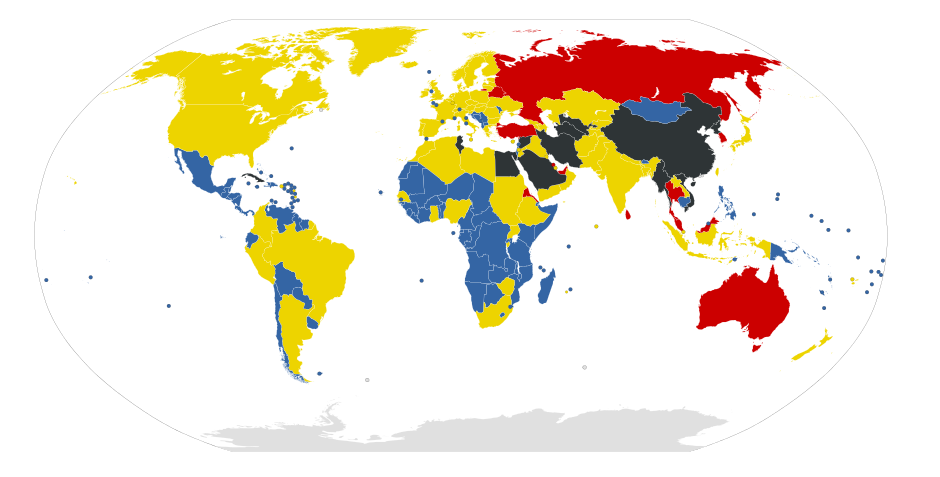
\includegraphics[scale=0.3]{Internet_blackholes}
\begin{tikzpicture}
\node at (0,0) [draw,fill,color=black,label=right:Zensiert] {};
\node at (0,-0.5) [draw,fill,color=red,label=right:Überwacht] {};
\node at (0,-1) [draw,fill,color=yellow,label=right:Teilweise zensiert] {};
\node at (0,-1.5) [draw,fill,color=blue,label=right:Freier Zugang] {};
\end{tikzpicture}
\end{block}
}

\section{Ziele von Freifunk}
\frame{
\frametitle{Ziele von Freifunk}
\begin{itemize}
 \item Gesellschaft vernetzen (freie Netze schaffen)
 \item Wissen verbreiten (Verschlüsselung, Technik)
 \item Keinen ausschließen
 \item Zensur erschweren
\end{itemize}
}

\section{Soziale Aspekte}
\frame{
\frametitle{Soziale Aspekte}
\begin{block}{Freie Kommunikation}
\begin{itemize}
 \item Sprache (Mumble)
 \item Text (Chat, IRC, Jabber)
 \item Web (Wiki)
\end{itemize}
\end{block}

\begin{block}{Zielgruppen}
\begin{itemize}
 \item Soziale Einrichtungen, Kirchen, Vereine
 \item Jedermann
\end{itemize}
\end{block}

\begin{block}{Bonus}
\begin{itemize}
 \item Internet-Sharing
\end{itemize}
\end{block}
}

\section{Technische Umsetzung}
\frame{
\frametitle{Technische Umsetzung}
\begin{block}{Teilnahme am Netz ist sehr einfach}
\begin{enumerate}
 \item WLAN-Router besorgen (meist vorhanden, neu: 15-50 Euro)
 \item Freifunk-Programm (Firmware) auf den Router laden
 \item Router aufstellen; sie bilden automatisch ein vermaschtes Funknetz
\end{enumerate}
\end{block}

\begin{block}{Nötiges Wissen}
Keins! Freifunker helfen, bzw. übernehmen die Arbeit.
\end{block}
}

\section{Rechtliche Aspekte}
\frame{
\frametitle{Rechtliche Aspekte}
\framesubtitle{Details: Extrafolien}
\begin{block}{Bei (mutmaßlichem) Missbrauch durch Nutzer}
\begin{itemize}
 \item Abmahnungen an den Betreiber
 \item Störerhaftung (Mindestschuld bei Klage)
 \item Besuch vom SEK
\end{itemize}
\end{block}

\begin{block}{Wunsch an Gesetzgeber}
Freifunkbetreiber wie Internetanbieter nicht für das Handeln ihrer Nutzer verantwortlich machen.
\end{block}
}

\section{Freifunk Rheinland e.V.}
\frame{
\frametitle{Freifunk Rheinland e.V.}
\begin{itemize}
 \item Gegründet: Ende 2010
 \item Gemeinnützig: Seit 21.03.2011
\end{itemize}

\begin{block}{Vereinssatzung}
\begin{quote}
Zweck des Vereins ist die Erforschung, Anwendung und Verbreitung freier Netzwerktechnologien sowie die Verbreitung und Vermittlung von Wissen über Funk und Netzwerktechnologien.
\end{quote}
\end{block}

\begin{block}{Funkzellen}
\begin{itemize}
 \item Lokale Gliederung mit eigenständiger Organisation.
 \item Hilfe des Vereins bei rechtlichen, organisatorischen und finanziellen Fragen.
\end{itemize}
\end{block}
}

\frame{
\frametitle{Freifunk Rheinland e.V.}
\begin{itemize}
 \item Routerpaten/Mietverträge
 \item Hilfestellung bei Technikfragen
 \item Regelmäßige Treffen und Workshops
\end{itemize}

\begin{block}{Mitgliedsbeitrag}
\begin{description}
 \item[voll] 5 Euro pro Monat
 \item[vermindert] 1 Euro pro Monat
\end{description}
\end{block}
}

\section{Mitmachen/Kontakt}
\frame{
\frametitle{Mitmachen/Kontakt}
\begin{block}{Kontakt zur Funkzelle Aachen}
\begin{framed}
An jedem ersten Dienstag des Monats um 19:30h in der Jülicher Str. 191 in Aachen, im Hackerspace des CCCAC.
\end{framed}
\end{block}

\begin{block}{Links zu Infos und Mailinglisten}
\begin{itemize}
 \item \url{http://aachen.freifunk.net/}
 \item \url{http://www.freifunk-rheinland.net/}
 \item \url{http://wiki.freifunk.net/}
 \item \url{http://start.freifunk.net/}
\end{itemize}
\end{block}
}
\end{document}